\documentclass[11pt,aspectratio=169]{beamer}

% -------------------- THEME & LAYOUT --------------------
\usetheme{Madrid}
\usecolortheme{dolphin} % base color scheme
\usefonttheme{professionalfonts}
\setbeamercovered{transparent}
\setbeamertemplate{navigation symbols}{}   % remove navigation buttons
\setbeamertemplate{caption}[numbered]      % numbered captions
\setbeamertemplate{itemize items}[triangle]
\setbeamersize{text margin left=1.2cm,text margin right=1.2cm} % adjust to taste
% -------------------- GLOBAL FONT SETTINGS --------------------

% 1. Force the base beamer font to small
\setbeamerfont{normal text}{size=\small}

% 2. Force math environments to follow the "small" font size
\setbeamerfont{math text}{size=\small}
\setbeamerfont{equation}{size=\small}

% 3. Redefine \normalsize itself 
% This ensures equations and lists (which look for \normalsize) use  instead.
\let\oldnormalsize\normalsize
\renewcommand{\normalsize}{\oldnormalsize\small}

% 4. Ensure lists also stay small
\setbeamerfont{itemize/enumerate body}{size=\small}
\setbeamerfont{itemize/enumerate subbody}{size=\small}
% -------------------- FONTS & TYPOGRAPHY --------------------
\usepackage[T1]{fontenc}
\usepackage[utf8]{inputenc}
\usepackage{newpxtext,newpxmath} % Palatino-like font & math
\usepackage{microtype}

% -------------------- MATH, TABLES & GRAPHICS --------------------
\usepackage{amsmath,amssymb,amsfonts,mathtools}
\usepackage{bm,booktabs,siunitx,graphicx}
\graphicspath{{./}{./figures/}}
%for eps figures
\usepackage{graphicx}
\usepackage{epstopdf}
%for numbered equations
\setcounter{equation}{0}
\renewcommand{\theequation}{10.\arabic{equation}}

% -------------------- UTILITIES --------------------
\usepackage{appendixnumberbeamer}
\usepackage{ragged2e}
\usepackage{xspace}
\usepackage{csquotes}
\usepackage{xcolor}

% -------------------- HYPERREF --------------------
\hypersetup{
  colorlinks=false,
  pdfauthor={Francesca},
  pdftitle={Chapter 1 — The Value of Currency}
}

% -------------------- COLORS & EMPHASIS --------------------
\definecolor{myblue}{RGB}{0,70,140}
\definecolor{myred}{RGB}{180,30,30}
\definecolor{mygreen}{RGB}{0,120,70}
\definecolor{gold}{RGB}{184,134,11}

\setbeamercolor{title}{fg=gold}       % title page
\setbeamercolor{frametitle}{fg=gold}  % slide titles
\setbeamercolor{structure}{fg=gold}   % bullets, sections, links
\setbeamercolor{section in head/foot}{fg=gold,bg=black!10} % gold text on light background

% -------------------- FOOTLINE --------------------
\setbeamertemplate{footline}{
  \leavevmode%
  \hbox{%
    % Section links (hidden if no current section)
    \begin{beamercolorbox}[wd=0.7\paperwidth,ht=2.5ex,dp=1.5ex,leftskip=1.4em]{section in head/foot}%
      \ifx\insertsection\empty
        % nothing
      \else
        Section: \insertsection
      \fi
    \end{beamercolorbox}%
    % Frame number right
    \begin{beamercolorbox}[wd=0.3\paperwidth,ht=2.5ex,dp=1.5ex,leftskip=3.8cm]{section in head/foot}%
      \insertframenumber/\inserttotalframenumber
    \end{beamercolorbox}%
  }%
  \vskip1pt%
}

\newcommand{\highlight}[1]{\textcolor{myblue}{#1}}
\newcommand{\warning}[1]{\textcolor{myred}{#1}}

% -------------------- SHORTCUTS --------------------
\newcommand{\E}{\mathbb{E}}
\newcommand{\R}{\mathbb{R}}
\newcommand{\dd}{\mathrm{d}}
\newcommand{\mc}[1]{\mathcal{#1}}
\newcommand{\bb}[1]{\mathbb{#1}}
\newcommand{\uc}{U_c}
\newcommand{\zg}{Z_g}

% -------------------- TIGHTER DISPLAY MATH --------------------
\makeatletter
\g@addto@macro\normalsize{%
  \setlength\abovedisplayskip{8pt}%
  \setlength\belowdisplayskip{8pt}%
  \setlength\abovedisplayshortskip{6pt}%
  \setlength\belowdisplayshortskip{6pt}%
}
\makeatother
\setbeamertemplate{frametitle}{
  \nointerlineskip
  \begin{beamercolorbox}[wd=\paperwidth,ht=3.5ex,dp=1ex,center]{frametitle}
    \centering\insertframetitle
  \end{beamercolorbox}
}

% -------------------- METADATA --------------------
\title[Part III — Crisis Models]{\textbf{Part II: Stabilization policies}\\[2pt]\large Chapter 10 - Deleveraging and Credit Crunch}
\author{Pierpaolo Benigno}
\institute{}
\date{\today}

% -------------------- SECTION ROADMAP --------------------
\AtBeginSection[]
{
  \begin{frame}
    \tableofcontents[currentsection, hideothersubsections]
  \end{frame}
}

% -------------------- Bibliography --------------------
\usepackage[backend=biber,style=authoryear]{biblatex}
\addbibresource{sources.bib}

\begin{document}

% ===================== TITLE SLIDE =====================
\begin{frame}[plain] % 'plain' removes header/footer for the title slide

\begin{columns}[T,totalwidth=\textwidth]

% ----- Left column: Main title, professor, chapter -----
\begin{column}{0.45\textwidth}
\vspace{2cm}

% Main title
{\usebeamercolor[fg]{title}\LARGE\textbf{Monetary Economics}\\[0.3cm]
\LARGE\textbf{and Policy}} 

\vspace{0.5cm}

% Professor name and date
{\large\textit{Pierpaolo Benigno}}\\[0.1cm]

\vspace{1cm}

% Chapter and subtitle
{\usebeamercolor[fg]{frametitle}\large Chapter 10: Deleveraging and Credit Crunch}

\end{column}

% ----- Right column: Image -----
\begin{column}{0.55\textwidth}
\vspace{1cm}
\centering

\includegraphics[width=0.9\linewidth]{Cover.png}
\end{column}

\end{columns}

% ----- Footer text (bottom-right corner) -----
\vspace*{2cm} % adjust if needed
\hfill{\large\textit{Prepared by Severin Rothen}}

\end{frame}

%-----------------------------------------------------------
%-----------------------------------------------------------
\begin{frame}{What We Will Learn}
\small
\begin{itemize}
  \item \textbf{Endogenous origins of liquidity traps:} How deleveraging and credit crunches can drive the natural real rate down (and potentially below zero), even without exogenous patience shocks.
  \item \textbf{Deleveraging mechanism:} Why forced repayment cuts borrowers’ spending and requires savers to spend more for goods markets to clear—lowering the natural rate.
  \item \textbf{Credit-crunch mechanism:} How banking stress tightens lending, widens credit spreads, and depresses demand—again pushing the natural rate down.
  \item How debt and spreads reshape the \textbf{aggregate demand (IS/AD) relation}, including Fisher debt-deflation versus borrowing-capacity effects.
  \item Why \textbf{sticky prices} and the \textbf{zero lower bound} can prevent the policy rate from falling enough, producing a Keynesian slump.
  \item What this implies for policy: why central banks must \textbf{monitor spreads} and may need \textbf{forward guidance} and \textbf{credit easing} to shorten liquidity traps.
\end{itemize}
\end{frame}

% OUTLINE
\begin{frame}{Outline}
\tableofcontents
\end{frame}

% =====================================================
\section{Introduction}
% =====================================================

%-----------------------------------------------------------
\begin{frame}{Liquidity Trap: Two Financial Mechanisms}
\small
\begin{itemize}
  \item Chapter~9 emphasized \textbf{exogenous preference shifts} (higher patience) as a driver of a low natural real rate, potentially pushing the economy into a liquidity trap.
  \vspace{0.4em}
  \item The post-2008 literature highlights additional \textbf{financial crisis mechanisms} that can also drive the natural real rate negative:
  \begin{enumerate}
    \item \textbf{Household debt deleveraging}.
    \item \textbf{Banking sector turbulence / credit crunch}.
  \end{enumerate}
\end{itemize}
\end{frame}

%-----------------------------------------------------------
\begin{frame}{Debt Deleveraging}
\small
\begin{itemize}
  \item Deleveraging typically follows a leveraging boom:
  \begin{itemize}
    \item Excessive optimism leads households to borrow and spend aggressively.
  \end{itemize}
  \vspace{0.3em}
  \item At the \textbf{``Minsky moment''} \parencite{EggertssonKrugman2012DebtDeleveragingLiquidityTrap},
  agents recognize that debt is unsustainable:
  \begin{enumerate}
    \item New borrowing stops.
    \item Overextended borrowers must repay (cut consumption).
  \end{enumerate}
  \vspace{0.3em}
  \item The demand for Full-employment then requires savers/creditors to spend more as debtors cut spending $\Rightarrow$ the \textbf{natural real rate falls}.
  \vspace{0.3em}
  \item If deleveraging is rapid, the natural real rate can become \textbf{negative}. With a limited ability to cut nominal rates, the \textbf{ZLB binds} and the output falls below potential.
\end{itemize}
\end{frame}

%-----------------------------------------------------------
\begin{frame}{Banking Turbulence and Credit Spreads}
\small
\begin{itemize}
  \item Interbank stress raises banks' funding costs, often reflecting:
  \begin{itemize}
    \item Capital losses.
    \item Leverage reductions / tighter regulatory or market constraints.
  \end{itemize}
  \vspace{0.3em}
  \item Tighter constraints make banks less willing to lend $\Rightarrow$ \textbf{credit crunch} and downturn.
  \vspace{0.3em}
  \item Banking turbulence (and deleveraging) typically widens \textbf{credit spreads}:
  \begin{itemize}
    \item Borrowing becomes more expensive than saving/lending.
    \item Private demand weakens.
  \end{itemize}
  \vspace{0.3em}
  \item To sustain demand at full employment, the \textbf{natural (risk-free) real rate must fall} to offset higher borrowing costs.
  \vspace{0.3em}
  \item Stabilization then requires a lower policy rate; at sufficiently large spreads, the economy risks hitting the \textbf{zero lower bound}.
\end{itemize}
\end{frame}

%-----------------------------------------------------------
\begin{frame}{Policy Implications of Credit Spreads}
\small
\begin{itemize}
  \item If the natural rate is shifted by credit spreads, policy must account for \textbf{credit-market conditions} (not only inflation and output gaps).
  \vspace{0.3em}
  \item Credit spreads are \textbf{endogenous}:
  \begin{itemize}
    \item Depend on macro conditions and balance-sheet strength (bank equity, borrower repayment capacity).
    \item Can amplify shocks via tighter lending conditions.
  \end{itemize}
  \vspace{0.3em}
  \item Monetary policy affects spreads through:
  \begin{enumerate}
    \item Conventional policy-rate cuts.
    \item At the ZLB, \textbf{unconventional credit easing} that improves balance sheets and compresses spreads.
  \end{enumerate}
  \vspace{0.3em}
  \item By limiting spread increases, policy prevents the natural rate from falling as much, reducing the likelihood and severity of a liquidity trap.
\end{itemize}
\end{frame}

\section{Outline of the Results}
\begin{frame}{Outline of the Results}
\small
\begin{itemize}
  \item The chapter develops a heterogeneous-agent New Keynesian model with two types of agents: \textit{savers} and \textit{borrowers}.
  \item A forced reduction in debt/loans (deleveraging or a credit contraction) can drive the \textbf{natural real rate} into negative territory.
  \item More generally, movements in the natural rate are driven by \textbf{credit-market spreads}, which in turn depend on macro-financial conditions and policy.
  \item Monetary policy can shorten liquidity traps, including through \textbf{unconventional credit easing}.
  \item Optimal policy is welfare-based and internalizes \textbf{distributional consequences} across agents.
\end{itemize}
\end{frame}


% =====================================================
\section{Debt Deleveraging}
% =====================================================

\begin{frame}{Preferences}
\small
    \begin{itemize}
        \item The economy is inhabited by savers $s$ and borrowers $b$, each receiving a constant endowment $\frac{1}{2}Y$ and with savers being more patient than borrowers $\beta^s > \beta^b$.
    \end{itemize}

\textbf{Expected Intertemporal Utility}
        \begin{equation}
            \E_{t_0}\sum_{t=t_0}^\infty (\beta^j)^{t-t_0}\log C_t^j, \qquad j\in\{s,b\}.
            \label{eq1}
        \end{equation}
\textbf{Flow Budget Constraint}
        \begin{equation}
            B_t^j = (1+r_{t-1})B_{t-1}^j - C_t^j + \frac{1}{2}Y, \qquad j\in\{s,b\}
            \label{eq2}
        \end{equation}
        
    \begin{itemize}
        \item $B_t^j$ are real assets and $r_{t-1}$ is the real interest rate set in period $t-1$.
    \end{itemize}
\end{frame}

\begin{frame}{Borrowing Limit and Euler Equation}
\small
\textbf{Borrowing Limit}
        \begin{equation}
            -(1+r_{t-1})B_{t-1}^j \le B^{high} \le \frac{1}{2}\frac{\beta}{1-\beta}Y.
        \end{equation}
    \begin{itemize}
        \item Outstanding debt and interest payment cannot exceed $B^{high}$, while $\frac{1}{2}\frac{\beta}{1-\beta}Y$ represents the maximum amount of debt that an agent can repay with certainty (see Chapter~1). 
        \item Note: We are setting $\beta^s = \beta$.
        \item Optimal consumption implies the Euler equation: 
        \begin{align}
            \frac{1}{C_t^j}\ge \beta^j(1+r_t)\E_t\!\left\{\frac{1}{C_{t+1}^j}\right\},
            \label{eq3}
        \end{align}
        which holds with inequality when the borrowing limit is binding at $t$.
    \end{itemize}
\end{frame}

\begin{frame}{Steady State}
\small
    \begin{itemize}
        \item Borrowers are less patient and therefore hit their borrowing limit. Equation~\eqref{eq2} together with the borrowing limit then implies:
        \begin{align*}
            C^b = \frac{1}{2}Y - \frac{r}{1+r}B^{high}.
        \end{align*}
       \vspace{1em} 
       \item Savers are unconstrained and therefore their Euler equation~\eqref{eq3} holds with equality. In steady state: $1 + r = \frac{1}{\beta^s}=\frac{1}{\beta}$. Moreover, since $C^b + C^s = Y$:
        \begin{align*}
            C^b = \frac{1}{2}Y + \frac{r}{1+r}B^{high}.
        \end{align*}
    \end{itemize}
\end{frame}

\begin{frame}{Deleveraging Shock}
\small
    \begin{itemize}
        \item Consider a shock at time $t$ that forces debtors to repay their debt so that $B^{high}$ goes to a lower threshold $B^{low}$ with $B^{high} > B^{low}$.
    \vspace{0.3em}
    \item At $t+1$ the economy reaches the new steady state (note that $\frac{r}{1+r} = 1-\beta$): 
        \begin{align*}
            C_{t+1}^b=\frac{1}{2}Y-(1-\beta)B^{low}, \quad
C_{t+1}^s=\frac{1}{2}Y+(1-\beta)B^{low}.
        \end{align*}
      \vspace{0.3em}
      \item Using the flow budget constraint~\eqref{eq2} and goods market equilibrium $C^b + C^s = Y$ we can obtain consumption at time $t$:
        \begin{align*}
            C_t^b=\frac{1}{2}Y+\frac{B^{low}}{1+r_t}-B^{high}, \quad
            C_t^s=\frac{1}{2}Y+B^{high}-\frac{B^{low}}{1+r_t}.
        \end{align*}
    \end{itemize}
\end{frame}

% Intuition: borrowers must reduce debt from $B^{high}$ to $B^{low}$, cutting spending.
% Savers must \highlight{consume more} to offset borrowers' deleveraging.

%-----------------------------------------------------------
\begin{frame}{The Short-Run Real Rate}
\small
\begin{itemize}
  \item Using the savers' Euler equation~\eqref{eq3} between $t$ and $t+1$, the market-clearing (natural) short-run real rate is:
  \begin{align*}
    1+r_t
    &= \frac{1}{\beta}\,
       \frac{\frac{1}{2}Y+B^{low}}{\frac{1}{2}Y+B^{high}}
    \;<\;\frac{1}{\beta}.
  \end{align*}
  \item Hence $r_t$ falls relative to its initial value and, for a sufficiently large deleveraging shock,
  \[
    \beta B^{high}-B^{low}>\frac{Y(1-\beta)}{2\beta},
  \]
  the natural real rate becomes negative.
  \vspace{0.3em}
  \item \textbf{Intuition:} Deleveraging forces borrowers to cut consumption (increase saving).  
  To keep output at full capacity, savers must be induced to absorb the excess supply of goods by consuming more, which requires a \emph{lower} real interest rate.
\end{itemize}
\end{frame}

%-----------------------------------------------------------
\begin{frame}{Zero Lower Bound}
\small
\begin{itemize}
  \item The $r_t$ derived above is the \textbf{frictionless market-clearing} (natural) real rate.
  \item With nominal rigidities, the actual real rate may not fall enough to match the natural rate.
  \item If the natural real rate turns negative, a nominal policy rate constrained by the ZLB, $i_t\ge 0$, can be too high in real terms:
  \begin{align*}
    r_t \;\approx\; i_t - \E_t\pi_{t+1}.
  \end{align*}
  \item \textbf{Consequence:} Insufficiently low real rates with respect to the natural rate of interest depress aggregate demand, producing a Keynesian slump (output falls below potential).
\end{itemize}
\end{frame}
% =====================================================
\section{Deleveraging with Endogenous Output and Sticky Prices}
% =====================================================
%-----------------------------------------------------------
\begin{frame}{Preferences}
\small
\begin{itemize}
  \item The economy is populated by two types of agents:
  \begin{itemize}
    \item \textbf{Savers $s$}: mass $\chi$,
    \item \textbf{Borrowers $b$}: mass $1-\chi$.
  \end{itemize}
  \vspace{0.4em}
\end{itemize}
\textbf{Intertemporal Utility}
  \begin{equation}
    \E_{t_0}\sum_{t=t_0}^\infty \beta^{\,t-t_0}\Big(U(C_t^j)-H(L_t^j)\Big), \qquad j\in\{s,b\}.
    \label{eq4}
  \end{equation}
\begin{itemize}
    \item $U(\cdot)$ is concave in consumption $C$,
    \item $H(\cdot)$ is convex in labor $L$.
  \item We adopt exponential utility in consumption:
  \begin{equation*}
    U(C_t^j)=1-\exp(-z\,C_t^j), \qquad z>0.
  \end{equation*}
\end{itemize}
\end{frame}

%-----------------------------------------------------------
\begin{frame}{Flow Budget Constraint}
\small
\textbf{Flow Budget Constraint}
  \begin{align}
    B_t^j
    =(1+i_{t-1})B_{t-1}^j
    -P_t C_t^j
    +W_t^j L_t^j
    +\Psi_t
    -T_t^j.
    \label{eq5}
  \end{align}
\textbf{Interpretation:}
  \begin{itemize}
    \item $B_t^j$ is the nominal position in one-period risk-free bonds.
    \item $i_{t-1}$ is the nominal interest rate.
    \item $P_t$ is the price level.
    \item $W_t^j$ and $L_t^j$ are the wage and labor of type $j$.
    \item $\Psi_t$ denotes firms' profits (distributed equally across agents).
    \item $T_t^j$ are lump-sum taxes.
  \end{itemize}
\end{frame}
\begin{frame}{Safe-Debt Threshold}
\begin{itemize}
  \item As before, there is a threshold below which debt can be treated as \textbf{safe}:
  \begin{align}
    -(1+r_t)\frac{B_t^j}{P_t}\le \bar{B},
    \label{eq6}
  \end{align}
  where $r_t$ is the real interest rate. 
  \item We assume that the safe-debt limit tightens at time $t$:
  \[
    \bar{B}:\; B^{high}\ \longrightarrow\ B^{low}.
  \]
\end{itemize}
\end{frame}

%-----------------------------------------------------------
\begin{frame}{Linearized Euler Equation}
\small
\begin{itemize}
  \item Households choose consumption and labor to maximize utility~\eqref{eq4}
  subject to the flow budget constraint~\eqref{eq5}, taking into account the
  debt limit~\eqref{eq6}.
  \vspace{0.3em}
  \item For savers, under perfect foresight, the Euler equation is
  \[
    \exp(-zC_t^s)=\beta(1+i_t)\frac{P_t}{P_{t+1}}\exp(-zC_{t+1}^s).
  \]
  \item Taking logs and rearranging yields
  \begin{align}
    C_t^s
    = C_{t+1}^s
    - \tilde{\sigma}\Big[\ln(1+i_t)-\pi_{t+1}-\tilde{\beta}\Big],
    \label{eq7}
  \end{align}
  where $\pi_{t+1}\equiv \ln(P_{t+1}/P_t)$, $\tilde{\beta}\equiv -\ln\beta$,
  and $\tilde{\sigma}\equiv 1/z$.
  \vspace{0.3em}
  \item \textbf{Remark:} With exponential utility, consumption enters in \emph{levels} (not logs) in~\eqref{eq7}.
\end{itemize}
\end{frame}

%-----------------------------------------------------------
\begin{frame}{AD Equation (Aggregation)}
\small
\begin{itemize}
  \item Using the aggregate resource constraint
  \[
    Y_t=\chi C_t^s+(1-\chi)C_t^b,
  \]
  substitute~\eqref{eq7} to obtain the aggregate demand (AD) relation:
  \begin{align*}
    Y_t
    &= Y_{t+1}
    -\chi\tilde{\sigma}\Big[\ln(1+i_t)-\pi_{t+1}-\tilde{\beta}\Big]
    +(1-\chi)\big(C_t^b-C_{t+1}^b\big).
  \end{align*}
  \vspace{0.2em}
  \item Expressing the equation in log deviations from steady state gives:
  \begin{align}
    \hat{Y}_t
    = \hat{Y}_{t+1}
    - \chi\sigma\Big[\hat{\imath}_t-(\pi_{t+1}-\pi)\Big]
    + (1-\chi)\left(\frac{C_t^b-C_{t+1}^b}{Y}\right),
    \label{eq8}
  \end{align}
  where $\hat{Y}_t\equiv \ln(Y_t/Y)$ and
  \[
    \hat{\imath}_t\equiv \ln\!\Big(\tfrac{1+i_t}{1+i}\Big),
    \qquad \ln(1+i)=\tilde{\beta}+\pi,
    \qquad \sigma\equiv \frac{\tilde{\sigma}}{Y}=\frac{1}{zY}.
  \]
\end{itemize}
\end{frame}

%--------------------------------------------------------%-----------------------------------------------------------
\begin{frame}{AD Equation (Borrower Deleveraging Term)}
\small
\begin{itemize}
  \item The borrower term $(C_t^b-C_{t+1}^b)$ shifts aggregate demand:
  \begin{itemize}
    \item Deleveraging lowers borrowers' short-run consumption $\Rightarrow$ AD falls even if interest rates are unchanged.
  \end{itemize}

  \vspace{0.35em}
  \item \textbf{Assumptions:} Borrowers are always at the debt limit
  $\bar B:\ B^{high}\to B^{low}$ at $t$, the real rate equals $r$ from $t+1$ onward,
  and $W_t^jL_t^j+\Psi_t=P_tY_t$ for all $t$.

  \vspace{0.35em}
  \item Borrower consumption (from~\ref{eq5}):
\[
\begin{aligned}
C_t^b
&= -\frac{1+i_{t-1}}{1+r_{t-1}}\frac{P_t}{P_{t-1}}\,B^{high}
  +\frac{B^{low}}{1+r_t}
  +Y_t-T_t^b,\\[0.3em]
C_{t+1}^b
&= -\frac{1+i_t}{1+r_t}\frac{P_{t+1}}{P_t}\,B^{low}
  +\frac{B^{low}}{1+r}
  +Y_{t+1}-T_{t+1}^b.
\end{aligned}
\]
\end{itemize}
\end{frame}


%-----------------------------------------------------------
\begin{frame}{AD Equation}
\small
\begin{itemize}
  \item Approximating the borrower-consumption expressions around the initial debt position
  and substituting into~\eqref{eq8} yields the short-run AD equation:
  \begin{align}
    \hat{Y}_{t}
    &= \E_t\hat{Y}_{t+1}
    -\varphi_{r}\Big[\hat{\imath}_{t}-(p_{t+1}-p_t-\pi)\Big]
    +\frac{1-\chi}{\chi}\Big[\hat{b}_{t}+b(p_t-p^\ast)\Big]
    -\frac{1-\chi}{\chi}\big(\hat{T}_{t}^{b}-\E_t\hat{T}_{t+1}^{b}\big),
    \label{eq9}
  \end{align}
  where
  \[
    \varphi_r \equiv \frac{\sigma\chi+(1-\chi)b\beta}{\chi}\ge 0,
    \qquad
    b \equiv \frac{B^{high}}{Y},
    \qquad
    \hat b_t \equiv \frac{B^{low}-B^{high}}{Y},
    \qquad
    \hat T_t^b \equiv \frac{T_t^b-T^b}{Y}.
  \]
  \item Here $Y$ is steady-state output, $p_t$ is the log price level, and inflation is $\pi_t\equiv p_t-p_{t-1}$ (with target $\pi$).
\end{itemize}
\end{frame}

%-----------------------------------------------------------
\begin{frame}{How Debt Changes the Slope of AD}
\small
\begin{itemize}
  \item Relative to the benchmark AD curve (Chapter~6), debt introduces \textbf{two opposing forces} that affect the slope of AD in $(p_t,y_t)$ space:
  \begin{enumerate}
    \item \textbf{Real-rate / borrowing-capacity channel:}
    higher $p_t$ raises the real rate, tightens the borrowing constraint, reduces $C_t^b$, and lowers demand.
    \begin{itemize}
      \item This increases $\varphi_r$ and tends to \textbf{flatten} AD.
    \end{itemize}
    \vspace{0.35em}
    \item \textbf{Fisher debt-deflation channel} (\cite{fisher1933}):
    higher $p_t$ reduces the real value of nominal debt, raises borrowers' net worth, increases $C_t^b$, and raises demand.
    \begin{itemize}
      \item This adds the term $\frac{1-\chi}{\chi}\,b\,(p_t-p^\ast)$ and tends to \textbf{steepen} AD.
    \end{itemize}
  \end{enumerate}
  \vspace{0.2em}
  \item \textbf{Net effect:} If the Fisher channel dominates, AD becomes \textbf{steeper} than in the previous model.
\end{itemize}
\end{frame}
%-----------------------------------------------------------
\begin{frame}{Labor Supply: Intratemporal Condition}
\small
\begin{itemize}
  \item For each type $j\in\{s,b\}$, labor supply satisfies the intratemporal condition
  (MRS between labor and consumption equals the real wage):
  \begin{align}
    \frac{H_l(L_t^j)}{U_c(C_t^j)}=\frac{W_t^j}{P_t}.
    \label{eq10}
  \end{align}

  \vspace{0.35em}
  \item \textbf{Functional forms.} Assume isoelastic disutility of work and exponential utility of consumption:
  \[
    H(L^j)=\frac{(L^j)^{1+\eta}}{1+\eta}
    \ \Rightarrow\ 
    H_l(L_t^j)=(L_t^j)^\eta,
    \qquad
    U(C^j)=1-e^{-zC^j}
    \ \Rightarrow\ 
    U_c(C_t^j)=z e^{-zC_t^j}.
  \]
  \item Hence, for each $j$,
  \[
    \frac{(L_t^j)^\eta}{z\,e^{-zC_t^j}}=\frac{W_t^j}{P_t}.
  \]
\end{itemize}
\end{frame}

%-----------------------------------------------------------
\begin{frame}{Labor Supply: Aggregation}
\small
\begin{itemize}
  \item \textbf{Aggregation.} Output is produced with
  \[
    Y_t=A_t L_t,
    \qquad
    L_t=(L_t^s)^\chi (L_t^b)^{1-\chi},
  \]
  and the corresponding aggregate wage index is
  \[
    W_t=(W_t^s)^\chi (W_t^b)^{1-\chi}.
  \]
  \item Taking a weighted average of the two intratemporal conditions (for $j=s,b$) with weights $\chi$ and $1-\chi$ gives the aggregate labor-supply schedule:
  \begin{equation}
    \frac{L_t^\eta}{z\exp\!\big[-z(\chi C_t^s+(1-\chi)C_t^b)\big]}
    =\frac{W_t}{P_t}.
    \label{ITLL}
  \end{equation}

  \item Using goods-market clearing $Y_t=\chi C_t^s+(1-\chi)C_t^b$ and production $Y_t=A_tL_t$, \eqref{ITLL} simplifies to:
  \begin{equation}
    \frac{(Y_t/A_t)^\eta}{z\exp(-zY_t)}=\frac{W_t}{P_t}.
    \label{eq12}
  \end{equation}
\end{itemize}
\end{frame}


%-----------------------------------------------------------
\begin{frame}{Natural Output}
\small
\begin{itemize}
  \item Under flexible prices, firms set a markup over marginal cost:
  \[
    P_t=\mu_t\,\frac{W_t}{A_t}.
  \]
  \vspace{0.35em}
  \item Combining this with \eqref{eq12}, the natural level of output $Y_t^n$ is implicitly defined by:
  \[
    \frac{\left(\frac{Y_t^n}{A_t}\right)^{\eta}}{z\exp(-zY_t^n)}
    =\frac{A_t}{\mu_t}.
  \]
  \vspace{0.35em}
  \item \textbf{Log-linear approximation (Chapter~5, with $G_t=0$):}
  \[
    \hat{Y}_t^{n}
    =\frac{1+\eta}{\sigma^{-1}+\eta}\hat{A}_t
    -\frac{1}{\sigma^{-1}+\eta}\hat{\mu}_t.
  \]
\end{itemize}
\end{frame}

%-----------------------------------------------------------
\begin{frame}{AS \& AD Equations}
\small
\begin{itemize}
  \item Given the natural output definition, the AS block is the same as in Chapter~5 (NKPC):
  \[
    \pi_t-\pi
    =\kappa(\hat Y_t-\hat Y_t^n)
    +\beta E_t(\pi_{t+1}-\pi),
  \]
  with
  \[
    \kappa \equiv \frac{1-\alpha}{\alpha}(1-\alpha\beta)\,
    \frac{\sigma^{-1}+\eta}{1+\theta\eta}.
  \]
  \vspace{0.35em}
  \item For tractability, assume $\pi_T=\pi$ for all $T\ge t+1$.
  \begin{itemize}
    \item Then $\hat Y_T=\hat Y_T^n$ for all $T\ge t+1$.
  \end{itemize}
  \vspace{0.35em}
  \item Under these assumptions, the time-$t$ AD schedule is upward sloping and can be written as:
  \[
    \hat{Y}_t
    = \hat{Y}_{t+1}^{n}
    - \varphi_r\,\hat{r}_t
    - \frac{1-\chi}{\chi}\big(\hat{\tau}_t^{b}-\hat{T}_{t+1}^{b}\big)
    + \frac{1-\chi}{\chi}\Big[\hat{b}_t + b\big(p_t-p^{*}\big)\Big].
  \]
\end{itemize}
\end{frame}

%--------------------------------------------------------

%-----------------------------------------------------------
\begin{frame}{Deleveraging Shock}
\begin{columns}[T,totalwidth=\textwidth]
\small

% -------- Left column: figure --------
\begin{column}{0.50\textwidth}
\centering
\vspace{-0.2cm}
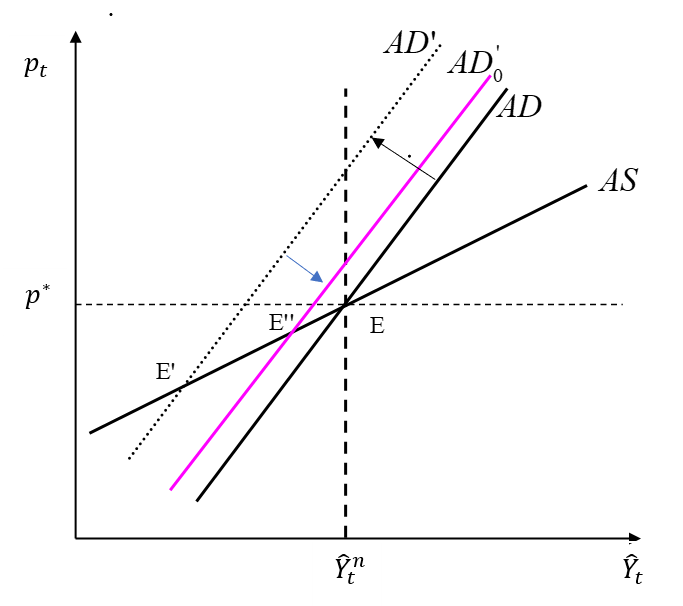
\includegraphics[width=\linewidth]{Figure22}
\vspace{-0.15cm}
{\scriptsize Deleveraging shifts $AD$ left ($E\to E'$). Cutting $i_t$ can move the economy to $E''$, but may be limited by the ZLB.}
\end{column}

% -------- Right column: description --------
\begin{column}{0.50\textwidth}
\small
\begin{flushright}
\begin{itemize}
  \item Deleveraging is a \textbf{left shift} of $AD$ (in~\eqref{eq9}: $\hat b_t<0$): $E\to E'$, with \textbf{lower output and prices}.
  \vspace{0.2em}
  \item Lowering the policy rate helps, but at the ZLB conventional policy may only move the economy to $E''$ (still below the initial allocation).
  \vspace{0.2em}
  \item \textbf{Paradox of thrift:} when borrowers try to save more, AD falls and output contracts, so \emph{aggregate} saving can fall.
  \parencite{EggertssonKrugman2012DebtDeleveragingLiquidityTrap}
\end{itemize}
\end{flushright}
\end{column}

\end{columns}
\end{frame}

%-----------------------------------------------------------
\begin{frame}{Paradox of ``Toil''}
\begin{columns}[T,totalwidth=\textwidth]
\small

% -------- Left column: figure --------
\begin{column}{0.50\textwidth}
\centering
\vspace{-0.2cm}
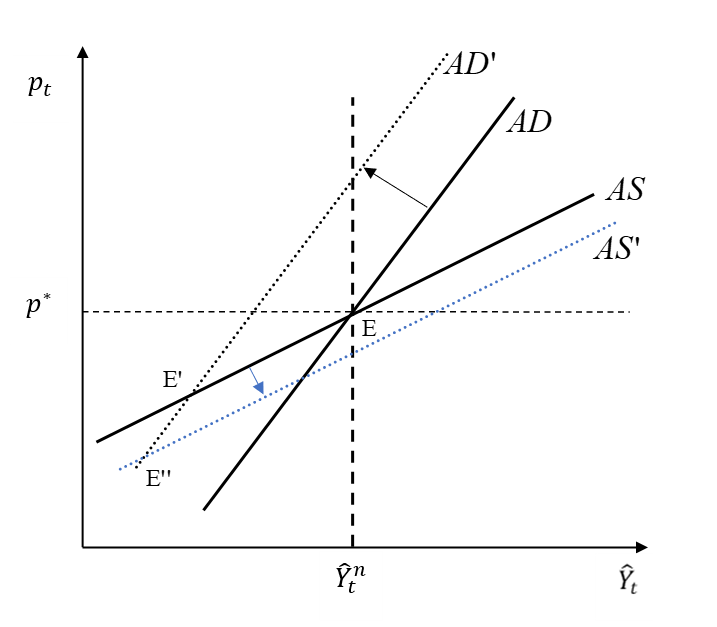
\includegraphics[width=\linewidth]{Figure23}
\vspace{-0.15cm}
{\scriptsize $AD$ shifts up ($E\to E'$). In a liquidity trap, a downward shift in $AS$ can be contractionary ($E'\to E''$).}
\end{column}

% -------- Right column: description --------
\begin{column}{0.50\textwidth}
\small
\begin{flushright}
\begin{itemize}
  \item In the liquidity-trap region, an \textbf{upward} shift in $AD$ moves equilibrium $E\to E'$.
  \vspace{0.2em}
  \item A \textbf{downward} shift in $AS$ can \emph{aggravate} the recession, moving equilibrium $E'\to E''$.
  \vspace{0.2em}
  \item This reversal is the \textbf{paradox of ``toil''}: changes that would normally raise output can become contractionary when monetary policy is constrained.
  \begin{itemize}
    \item Examples: temporary increase in productivity, or a fall in the markup.
  \end{itemize}
\end{itemize}
\end{flushright}
\end{column}

\end{columns}
\end{frame}

%-----------------------------------------------------------
\begin{frame}{Paradox of Flexibility and Escaping the Liquidity Trap}
\small

\textbf{Paradox of flexibility}
\begin{itemize}
  \item More flexible prices $\Rightarrow$ a \textbf{steeper} AS curve.
  \item With deleveraging, a steeper AS implies \textbf{larger output contractions}.
  \item The larger fall in prices raises the real value of nominal debt (debt-deflation), depressing demand further.
\end{itemize}

\vspace{0.6em}
\textbf{Escaping the liquidity trap}
\begin{itemize}
  \item \textbf{Raise the future price level} (see Chapter~9):
  \begin{itemize}
    \item Higher expected inflation lowers the real rate, easing deleveraging and stimulating savers' consumption.
    \item This channel is reinforced here because $\varphi_r$ in~\eqref{eq9} is larger than in the benchmark model.
  \end{itemize}
  \item Policies that \textbf{increase long-run output} are also expansionary (shift $AD$ to the right).
\end{itemize}
\end{frame}

% =====================================================
\section{Credit Crunch}
% =====================================================
%-----------------------------------------------------------
\begin{frame}{Credit Crunch: Banking-Sector Turbulence}
\small
\begin{itemize}
  \item Alternative post-2007/08 narrative: the recession is driven by \textbf{banking-sector stress} rather than (only) borrower deleveraging.
  \vspace{0.3em}
  \item Mechanism:
  \begin{itemize}
    \item Risky assets on intermediaries' balance sheets raise funding costs.
    \item Banks respond by raising equity and/or reducing leverage.
    \item Capital constraints tighten $\Rightarrow$ lending supply contracts.
    \item Lower credit availability depresses spending and output.
  \end{itemize}
  \vspace{0.3em}
  \item We capture this with an explicit \textbf{lending-supply limit} in the simplified framework of the previous section.
\end{itemize}
\end{frame}

%-----------------------------------------------------------
\begin{frame}{Modified Debt and Lending Limits}
\small
\begin{itemize}
  \item Two agents: savers and borrowers, with preferences~\eqref{eq1} and budget constraint~\eqref{eq2}.
  \vspace{0.3em}
  \item The debt constraint is augmented by an \textbf{upper bound on lending}:
  \begin{equation*}
    \mathrm{L}^{high}
    \;\ge\;
    (1+r_{t-1})B_{t-1}^j
    \;\ge\;
    -B^{high}
    \;\ge\;
    -\frac{1}{2}\frac{\beta}{1-\beta}Y.
  \end{equation*}
  \vspace{0.3em}
  \item Interpretation:
  \begin{itemize}
    \item $\mathrm{L}^{high}$: maximum credit that lenders are willing/able to supply,
    \item $B^{high}$: maximum borrowing capacity (``safe'' debt limit).
  \end{itemize}
  \vspace{0.3em}
  \item Initial steady state: $\mathrm{L}^{high}>B^{high}$, so the lending limit is slack (only the borrowing limit is relevant).
\end{itemize}
\end{frame}


%--------------------------------------------------------%-----------------------------------------------------------
\begin{frame}{Initial Steady State: Saving vs.\ Borrowing Rates}
\small
\begin{itemize}
  \item It is useful to distinguish between the \textbf{saver's} and the \textbf{borrower's} real rate.
  \vspace{0.1em}
  \item Savers are unconstrained, so their steady-state real rate is pinned down by the Euler equation:
  \[
    1+r^{s}=\frac{1}{\beta^{s}}=\frac{1}{\beta}.
  \]
  \vspace{0.1em}
  \item Borrowers are at the borrowing limit and therefore do not satisfy their Euler equation with equality.
  Define an implicit (shadow) borrowing rate by evaluating~\eqref{eq3} at steady-state borrower consumption:
  \[
    1+r^{b}=\frac{1}{\beta^{b}}
    \;>\;
    1+r^{s}.
  \]
  \item Hence there is a positive steady-state spread,
  \[
    r^{b}-r^{s}>0,
  \]
  capturing that borrowers are more impatient than savers.
\end{itemize}
\end{frame}


%-----------------------------------------------------------
\begin{frame}{Credit Crunch Shock}
\small
\begin{itemize}
  \item Banking-sector turbulence reduces the maximum lending supply from $\mathrm{L}^{high}$ to $\mathrm{L}^{low}$.
  \item If $\mathrm{L}^{low}<B^{high}$, savers become constrained and lending is pinned down by $\mathrm{L}^{low}$ (the supply limit binds).
  \vspace{0.3em}
  \item Long-run allocations (from $t+1$ onward):
  \[
    C_{t+1}^b=\frac{1}{2}Y-(1-\beta^b)\mathrm{L}^{low},
    \qquad
    C_{t+1}^s=\frac{1}{2}Y+(1-\beta^b)\mathrm{L}^{low}.
  \]
  \vspace{0.3em}
  \item Since savers are constrained, the \textbf{borrowers' discount factor} is the relevant one for pricing the long-run real rate.
\end{itemize}
\end{frame}

%-----------------------------------------------------------
\begin{frame}{Short Run (Time $t$)}
\small
\begin{itemize}
  \item Using the flow budget constraint~\eqref{eq2}, with initial asset position $B^{high}$ and long-run position $\mathrm{L}^{low}$, saver consumption at time $t$ is:
  \[
    C_t^s=\frac{1}{2}Y-\frac{\mathrm{L}^{low}}{1+r_t^b}+B^{high}.
  \]
  \vspace{0.25em}
  \item Market clearing implies $C_t^b+C_t^s=Y$, hence borrower consumption:
  \[
    C_t^b=\frac{1}{2}Y+\frac{\mathrm{L}^{low}}{1+r_t^b}-B^{high}.
  \]
  \vspace{0.25em}
  \item In the short run, the market real rate is $r_t^b$ because the borrowers' Euler equation holds with equality (they are marginal in pricing).
\end{itemize}
\end{frame}

%-----------------------------------------------------------
\begin{frame}{Borrowing Rate}
\small
\begin{itemize}
  \item Insert the short- and long-run borrower consumption into the Euler equation~\eqref{eq3} (holding with equality) to solve for the short-run borrowing rate:
  \[
    1+r_t^b=\frac{1}{\beta^b}\,
    \frac{\frac{1}{2}Y-\mathrm{L}^{low}}{\frac{1}{2}Y-B^{high}}
    \;>\;\frac{1}{\beta^b}.
  \]
  \vspace{0.3em}
  \item If $\mathrm{L}^{low}<B^{high}$, the borrowing rate \textbf{jumps up}.
  \begin{itemize}
    \item A negative lending-supply shock therefore raises the effective rate faced by borrowers.
  \end{itemize}
\end{itemize}
\end{frame}

%-----------------------------------------------------------
%-----------------------------------------------------------
\begin{frame}{Shadow Saving Rate}
\small
\begin{itemize}
  \item With a binding lending limit, savers cannot freely increase their asset holdings.
  Hence the savers' Euler condition (\ref{eq3}) holds with a \textbf{strict reverse inequality}:
  \[
    U_c(C_t^s)\;>\;\beta^s(1+r_t^b)\,U_c(C_{t+1}^s).
  \]
  

  \item Define the \textbf{shadow saving rate} $r_t^s$ as the interest rate that would make the savers' Euler equation hold with equality:
  \[
    U_c(C_t^s)=\beta^s(1+r_t^s)\,U_c(C_{t+1}^s).
  \]
  \item In the model, $r_t^s$ satisfies:
  \begin{align}
    1+r_t^s
    &= \frac{1}{\beta^s}\frac{\frac{1}{2}Y+\mathrm{L}^{low}}{\frac{1}{2}Y+B^{high}}
    +\frac{1}{\frac{1}{2}Y+B^{high}}
      \left(\frac{1+r_t^s}{1+r_t^b}-\frac{\beta^b}{\beta^s}\right)\mathrm{L}^{low}.
    \label{eq13}
  \end{align}

  \item The RHS is increasing in $(1+r_t^s)$ and lies below the $45^\circ$ line at $(1+r_t^s)=1/\beta^s$,
  implying the fixed point:
  \[
    1+r_t^s<\frac{1}{\beta^s}.
  \]
\end{itemize}
\end{frame}


%-----------------------------------------------------------
\begin{frame}{Intuition: Borrowing vs.\ Saving Rates}
\small
\begin{itemize}
  \item A contraction in credit supply raises the borrowing rate above its steady state:
  \[
    1+r_t^b>\frac{1}{\beta^b}.
  \]
  \item At the same time, the spread widens: $r_t^b-r_t^s$ increases when lending falls.
  \vspace{0.25em}
  \item In~\eqref{eq13}, the second term becomes negative, which pushes the shadow saving rate down:
  \[
    1+r_t^s \downarrow.
  \]
\end{itemize}
\textbf{Interpretation:}
\begin{itemize}
    \item Savers are forced to lend less, so they must be induced to \textbf{save less and consume more} $\Rightarrow$ lower $r_t^s$.
    \item Borrowers must \textbf{borrow less and consume less} to clear goods markets $\Rightarrow$ higher $r_t^b$.
  \item This mirrors the deleveraging case: borrowing rate increases while the saving rate falls.
\end{itemize}
\end{frame}

%-----------------------------------------------------------
\begin{frame}{Deleveraging and Credit Crunch: Isomorphism}
\small
\begin{itemize}
  \item Deleveraging shocks and credit-crunch shocks imply the same qualitative movements:
  \begin{itemize}
    \item $r_t^b$ rises to discourage borrowing and compress borrower spending,
    \item $r_t^s$ falls to encourage saver consumption,
    \item the spread $r_t^b-r_t^s$ widens.
  \end{itemize}
  \vspace{0.25em}
  \item A sufficiently large contraction can push the saving real rate below zero,
  potentially generating a liquidity trap.
  
\end{itemize}
\end{frame}

%-----------------------------------------------------------
\begin{frame}{Income Variation and the Interest Rate Spread}
\small
\begin{itemize}
  \item Credit spreads can also move because of income changes (not only borrowing/lending limits).
  \vspace{0.25em}
  \item \textbf{Temporary aggregate income increase} affecting both agents equally:
  \begin{itemize}
    \item Constrained borrowers consume the additional income.
    \item Savers would like to save more $\Rightarrow$ the saving rate must fall to stimulate their consumption.
    \item The shadow borrowing rate falls proportionally, so the spread is (approximately) unchanged.
  \end{itemize}
  \vspace{0.25em}
  \item \textbf{Unequal income changes / transfers} can change the spread:
  \begin{itemize}
    \item E.g.\ borrowers' income rises while savers' income falls.
    \item Borrowers consume the transfer, savers would like to borrow (reduce assets).
    \item Goods-market clearing requires the saving rate to rise (discourage savers from borrowing).
    \item The borrowing rate falls, so the spread decreases.
  \end{itemize}
\end{itemize}
\end{frame}

% =====================================================
\section{A General Framework}
% =====================================================

%-----------------------------------------------------------
\begin{frame}{Two Euler Equations with Default Risk}
\small
\begin{itemize}
  \item Consider again a two-agent economy with preferences given by~\eqref{eq4}.
  \item Savers and borrowers are \textbf{unconstrained}, so their Euler equations hold with equality.
  \vspace{0.25em}
  \item Saver Euler equation:
  \begin{align}
    \exp(-zC_t^s)
    =\beta^s(1+i_t^s)\E_t\!\left\{\frac{P_t}{P_{t+1}}\exp(-zC_{t+1}^s)\right\}.
    \label{eq14}
  \end{align}
  \item Borrower Euler equation with default risk:
  \begin{align}
    \exp(-zC_t^b)
    =\beta^b(1+i_t^b)\E_t\!\left\{\frac{P_t}{P_{t+1}}(1-\omega_{t+1})\exp(-zC_{t+1}^b)\right\},
    \label{eq15}
  \end{align}
  where $i_t^s$ and $i_t^b$ are nominal interest rates faced by savers and borrowers, and $\omega_{t+1}\in[\omega_{\min},\omega_{\max}]$ is the default rate with
  $0<\omega_{\min}<\omega_{\max}<1$.
\end{itemize}
\end{frame}

%-----------------------------------------------------------
\begin{frame}{Log-Linearization and Aggregation}
\small
\begin{itemize}
  \item A log-linear approximation of \eqref{eq14}--\eqref{eq15} yields:
  \[
    C_t^s=\E_t C_{t+1}^s-\frac{1}{z}\Big(\hat{\imath}_t^s-\E_t(\pi_{t+1}-\pi)\Big),
    \qquad
    C_t^b=\E_t C_{t+1}^b-\frac{1}{z}\Big(\hat{\imath}_t^b-\E_t\hat{\omega}_{t+1}-\E_t(\pi_{t+1}-\pi)\Big),
  \]
  where hats denote log-deviations and $\hat\omega_{t+1}$ is the deviation of the default rate from steady state.
  \vspace{0.25em}
  \item Using aggregation $Y_t=\chi C_t^s+(1-\chi)C_t^b$, we obtain:
  \begin{align}
    \hat{Y}_t
    =\E_t\hat{Y}_{t+1}
    -\sigma\Big(
      \hat{\imath}_t^s-\E_t(\pi_{t+1}-\pi)
      +(1-\chi)\big(\hat{\imath}_t^b-\E_t\hat{\omega}_{t+1}-\hat{\imath}_t^s\big)
    \Big),
    \label{eq16}
  \end{align}
  where $\sigma\equiv \frac{1}{zY}$.
\end{itemize}
\end{frame}

%-----------------------------------------------------------
\begin{frame}{Interest-Rate Spread as a Preference Shock}
\small
\begin{itemize}
  \item Equation~\eqref{eq16} is isomorphic to the Chapter~5 AD equation (with $G_t=0$).
  \vspace{0.25em}
  \item Identify the policy-relevant nominal rate with the saver rate:
  \[
    \hat{\imath}_t\equiv \hat{\imath}_t^s.
  \]
  \item The remaining wedge behaves like a preference (demand) shock:
  \[
    E_t\Delta\hat{\xi}_{t+1}
    \equiv
    E_t(\hat{\xi}_{t+1}-\hat{\xi}_t)
    =(1-\chi)\Big(\hat{\imath}_t^b-\E_t\hat{\omega}_{t+1}-\hat{\imath}_t^s\Big).
  \]
  \vspace{0.25em}
  \item Hence a higher \textbf{default-adjusted credit spread} lowers aggregate demand and output, exactly like a negative preference shock.
\end{itemize}
\end{frame}

%-----------------------------------------------------------
\begin{frame}{Natural (Efficient) Real Rate with Spreads}
\small
\begin{itemize}
  \item Rewrite AD in efficient-gap form (same $\hat Y_t^e$ as Chapter~7):
  \begin{align}
    \hat{Y}_t-\hat{Y}_t^{e}
    =\E_t(\hat{Y}_{t+1}-\hat{Y}_{t+1}^{e})
    -\sigma\Big(\hat{\imath}_t^s-\E_t(\pi_{t+1}-\pi)-r_t^{e}\Big).
    \label{eq17}
  \end{align}
  \vspace{0.25em}
  \item The frictionless (efficient) real rate is:
  \begin{align}
    r_t^{e}
    \equiv
    \E_t\!\left\{
      \frac{1+\eta}{1+\sigma\eta}\big(\hat{A}_{t+1}-\hat{A}_t\big)
      -(1-\chi)\big(\hat{\imath}_t^b-\E_t\hat{\omega}_{t+1}-\hat{\imath}_t^s\big)
    \right\}.
    \label{eq18}
  \end{align}
  \vspace{0.25em}
  \item A rise in the default-adjusted credit spread lowers $r_t^e$.
  \begin{itemize}
    \item If the spread is endogenous, monetary policy can influence $r_t^e$ indirectly through its effects on credit conditions.
  \end{itemize}
\end{itemize}
\end{frame}

%-----------------------------------------------------------
\begin{frame}{AS Equation}
\small
\begin{itemize}
  \item With exponential utility and Cobb--Douglas aggregation, the AS block takes the same reduced form as in Chapter~5/7:
  \begin{align}
    \pi_t-\pi
    =\kappa(\hat{Y}_t-\hat{Y}_t^{e})
    +\upsilon_t
    +\beta\E_t(\pi_{t+1}-\pi).
    \label{eq19}
  \end{align}
  \item The parameters $\kappa$ and $\upsilon_t$ are as defined earlier.
  \vspace{0.25em}
  \item \textbf{Key message:} Heterogeneity affects the \textbf{IS/AD side} through spreads, while the Phillips-curve structure remains standard.
\end{itemize}
\end{frame}

%-----------------------------------------------------------
\begin{frame}{Financial Intermediaries}
\small
\begin{itemize}
  \item A stylized intermediary (lives $t$ and $t+1$) lends $Z_t$, funded with deposits $D_t$ and equity $N_t$.
  Its balance-sheet constraint is:
  \begin{align}
    Z_t = D_t + N_t\big(1-\varsigma(Z_t)\big),
    \label{eq20}
  \end{align}
  where $\varsigma(Z_t)$ is an extra cost per unit of equity, non-decreasing in $Z_t$.
  \vspace{0.35em}
  \item At $t+1$, nominal profits are:
  \begin{align}
    \Psi_{t+1}^I
    =(1+i_t^b)(1-\omega_{t+1})Z_t-(1+i_t^s)D_t.
    \label{eq21}
  \end{align}
    \item Lending earns $i_t^b$ but faces random default $\omega_{t+1}$,
    \item Deposits pay the saving rate $i_t^s$.
\end{itemize}
\end{frame}

%-----------------------------------------------------------
\begin{frame}{Limited Liability and Equity Lower Bound}
\small
\begin{itemize}
  \item Limited liability requires $\Psi_{t+1}^I\ge 0$ in all states; in the worst case $\omega_{\max}$:
  \begin{align}
    (1+i_t^b)(1-\omega_{\max})Z_t \ge (1+i_t^s)D_t.
    \label{eq22}
  \end{align}
  \vspace{0.25em}
  \item Using \eqref{eq20} to substitute for $D_t$ gives:
  \[
    \Big[(1+i_t^b)(1-\omega_{\max})-(1+i_t^s)\Big]Z_t
    \ge -(1+i_t^s)\,N_t\big(1-\varsigma(Z_t)\big).
  \]
  \vspace{0.25em}
  \item Equivalently, equity must satisfy the lower bound:
  \begin{align}
    N_t \ge \frac{1}{1-\varsigma(Z_t)}
    \left[1-\frac{1+i_t^b}{1+i_t^s}(1-\omega_{\max})\right]Z_t.
    \label{eq23}
  \end{align}
  \item Intuition: intermediaries must hold enough equity to absorb losses under worst-case default.
\end{itemize}
\end{frame}

%-----------------------------------------------------------
\begin{frame}{Intermediary Rents}
\small
\begin{itemize}
  \item Intermediaries are owned by savers and maximize rents:
  \[
    \mathcal{R}_t
    =E_t\!\left\{\tilde{R}^{\,s}_{t,t+1}\,\Psi^I_{t+1}\right\}-N_t,
  \]
  where the saver SDF is
  \[
    \tilde{R}^{\,s}_{t,t+1}
    =\beta^s\frac{\exp(-zC_{t+1}^s)}{\exp(-zC_t^s)}\frac{P_t}{P_{t+1}}.
  \]
  \vspace{0.25em}
  \item Using \eqref{eq21} and the saver Euler equation \eqref{eq14}, rents can be written as:
  \begin{align}
    \mathcal{R}_t
    =\frac{1+i_t^b}{1+i_t^s}\Big(1-\tilde{E}_t\omega_{t+1}\Big)Z_t
    -D_t-N_t,
    \label{eq24}
  \end{align}
  where expected default is measured under the ``risk-neutral'' probability:
  \begin{align}
    \tilde{E}_t\omega_{t+1}
    \equiv (1+i_t^s)\,E_t\!\left\{\tilde{R}^{\,s}_{t,t+1}\,\omega_{t+1}\right\}.
    \label{eq25}
  \end{align}
\end{itemize}
\end{frame}


%-----------------------------------------------------------
\begin{frame}{Zero Rents and the Interest-Rate Spread}
\small
\begin{itemize}
  \item Substitute $D_t$ from the balance sheet~\eqref{eq20} into rents~\eqref{eq24}:
  \[
    \mathcal{R}_t
    =\left(\frac{1+i_t^b}{1+i_t^s}\left(1-\tilde{E}_t\omega_{t+1}\right)-1\right)Z_t
    -\varsigma(Z_t)\,N_t .
  \]
  \vspace{0.25em}
  \item Impose limited liability~\eqref{eq23} with equality to eliminate $N_t$, obtaining:
  \begin{align}
    \mathcal{R}_t
    = Z_t\Bigg[
      \left(\frac{1+i_t^b}{1+i_t^s}\left(1-\tilde{E}_t\omega_{t+1}\right)-1\right)
      -\frac{\varsigma(Z_t)}{1-\varsigma(Z_t)}
      \left(1-\frac{1+i_t^b}{1+i_t^s}(1-\omega_{\max})\right)
    \Bigg].
    \label{eq26}
  \end{align}
  \vspace{0.25em}
  \item Competition implies $\mathcal{R}_t=0$, pinning down the spread:
  \begin{align}
    \frac{1+i_t^b}{1+i_t^s}
    = \frac{1}{(1-\varsigma(Z_t))\left(1-\tilde{E}_t\omega_{t+1}\right)
    + \varsigma(Z_t)\left(1-\omega_{\max}\right)}.
    \label{eq27}
  \end{align}
\end{itemize}
\end{frame}

%-----------------------------------------------------------
\begin{frame}{Equity-to-Loans Ratio}
\small
\begin{itemize}
  \item Using \eqref{eq23} and the spread condition \eqref{eq27}, the equity-to-loans ratio is:
  \[
    \frac{N_t}{Z_t}
    =\frac{1+i_t^b}{1+i_t^s}\left(\omega_{\max}-\tilde{E}_t\omega_{t+1}\right).
  \]
  \vspace{0.25em}
\end{itemize}
\textbf{Interpretation
}  
\begin{itemize}
    \item $\frac{N_t}{Z_t}$ increases with the spread and with the gap between worst-case and expected loan losses.
    \item Intermediaries must hold equity to cover losses under the worst-case default scenario.
  \end{itemize}
\textbf{Special case:}
\begin{itemize}
  \vspace{0.25em}
  \item If $\varsigma(\cdot)=0$, then \eqref{eq27} depends only on expected default risk.
  In a log-linear approximation, this is not a (first-order) source of perturbation in the AD equation~\eqref{eq16}.
\end{itemize}
\end{frame}

%-----------------------------------------------------------
\begin{frame}{Spread Function}
\small
\begin{itemize}
  \item The spread can be summarized as a reduced-form function:
  \[
    \frac{1+i_t^b}{1+i_t^s}
    = s\!\left(Z_t,\omega_{\max},\tilde{E}_t\omega_{t+1}\right).
  \]
  \vspace{0.25em}
  \item Comparative statics:
  \begin{itemize}
    \item $s(\cdot)$ is non-decreasing in $Z_t$ if $\varsigma(Z_t)$ is non-decreasing (higher intermediation increases equity-raising costs).
    \item Higher $\varsigma(Z_t)$ increases the spread.
    \item Higher worst-case loss $\omega_{\max}$ or higher expected loss $\tilde{E}_t\omega_{t+1}$ increases the spread.
  \end{itemize}
\end{itemize}
\end{frame}

%-----------------------------------------------------------
\begin{frame}{Model Implications and Extensions}
\small
\begin{itemize}
  \item The stylized model is consistent with broader mechanisms:
  \begin{itemize}
    \item Higher intermediation volumes require a higher spread to compensate for risk and equity costs.
    \item The worst-case default rate $\omega_{\max}$ can be endogenized (e.g.\ as a function of borrower income or collateral values).
    \item In good macro states, a lower $\omega_{\max}$ reduces spreads.
  \end{itemize}
  \vspace{0.25em}
  \item These channels highlight the interaction between spreads, policy, and macro outcomes, motivating richer models of spread determination.
  \vspace{0.25em}
  \item Examples where spreads depend on aggregate debt and interact with monetary policy:
  \textcite{BenignoEtAl2020} and \textcite{CurdiaWoodford2010,CurdiaWoodford2011}.
\end{itemize}
\end{frame}


% =====================================================
\section{Policy Implications}
% =====================================================

%-----------------------------------------------------------
\begin{frame}{Why Policy Must Watch Credit Spreads}
\small
\begin{itemize}
  \item From \eqref{eq17}--\eqref{eq18}:
  \begin{itemize}
    \item Stabilization requires moving the policy-relevant rate $i_t^s$ in line with the efficient real rate $r_t^{e}$.
    \item If the default-adjusted spread rises, $r_t^{e}$ \textbf{falls} even absent preference shocks.
    \item Therefore the policy rate must fall by \textbf{more}; at the ZLB this may be impossible.
  \end{itemize}
  \vspace{0.25em}
  \item \textbf{Conclusion:} Credit spreads provide real-time information about the ``right'' real rate and the stance of policy.
\end{itemize}
\end{frame}

%-----------------------------------------------------------
\begin{frame}{Forward Guidance with Endogenous Spreads}
\small
\begin{itemize}
  \item Chapter~9: Forward guidance (guidance about future short rates) helps escape a liquidity trap.
  \vspace{0.25em}
  \item With endogenous spreads, the exit from ZLB policies can occur earlier than when the disturbance is purely exogenous:
  \begin{itemize}
    \item Policies that improve borrowers' repayment capacity can shorten deleveraging.
    \item Policies that reduce default probabilities can dampen the initial banking shock and its propagation.
  \end{itemize}
  \vspace{0.25em}
  \item Endogenous spreads can also attenuate the sensitivity of output to movements in $\hat{\imath}_t^s$.
\end{itemize}
\end{frame}

%-----------------------------------------------------------
\begin{frame}{Optimal Policy}
\small
\begin{itemize}
  \item A second-order approximation of welfare around the efficient steady state yields the quadratic loss:
  \begin{align}
    L_{t_0}^{CB}
    =\frac{1}{2}\E_{t_0}\!\left\{\sum_{t=t_0}^\infty \beta^{t-t_0}\left[
      (\hat{Y}_t-\hat{Y}_t^{e})^2
      +\chi(1-\chi)\Lambda_c(\hat{C}_t^b-\hat{C}_t^s)^2
      +\Lambda_\pi(\pi_t-\pi)^2
    \right]\right\}.
    \label{eq28}
  \end{align}
  \vspace{0.15em}
  \item Relative to Chapter~7, policy now also cares about \textbf{risk sharing}:
  deviations $(\hat C_t^b-\hat C_t^s)$ capture distributional distortions across borrowers and savers.
  \vspace{0.25em}
  \item Even with exogenous spreads, policy should account for financial conditions
  (\cite{CurdiaWoodford2016}).
  \item With deleveraging or banking turbulence, distributional concerns tilt optimal policy in a more expansionary direction (supporting borrowers' consumption).
\end{itemize}
\end{frame}

%-----------------------------------------------------------
\begin{frame}{Unconventional Monetary Policy}
\small
\begin{itemize}
  \item The framework supports \textbf{credit-easing} policies (Chapter~9):
  they can compress credit spreads and mitigate the decline in the efficient real rate during crises.
  \vspace{0.25em}
  \item Acting as lender of last resort, the central bank can counteract spread widening,
  dampening the impact of financial distress on inflation and output.
  \vspace{0.25em}
  \item Credit easing can help achieve output and inflation objectives and reduce both the \textbf{severity} and the \textbf{duration} of a liquidity trap.
\end{itemize}
\end{frame}

% =====================================================
\section{Summary}
% =====================================================

%-----------------------------------------------------------
\begin{frame}{Main Takeaways}
\small
\begin{itemize}
  \item \textbf{Liquidity traps can be endogenous:} Deleveraging and credit crunches lower the natural real rate and can push it below zero.
  \item \textbf{Deleveraging:} Borrowers cut spending; full-employment demand requires savers to spend more, implying a lower natural rate.
  \item \textbf{Credit crunch:} Banking stress tightens lending and widens credit spreads, depressing demand and lowering the efficient real rate.
  \item With \textbf{sticky prices} and the \textbf{ZLB}, the policy rate may not fall enough, generating a Keynesian slump and debt-deflation dynamics.
  \item \textbf{Policy lesson:} Monitor spreads and use forward guidance / credit easing to compress spreads and shorten liquidity traps.
\end{itemize}
\end{frame}



% =====================================================
\section{Bibliography}
% =====================================================

\begin{frame}{References}
\printbibliography
\end{frame}

\end{document}
